\subsection{Amélioration de la factorisation et de la résolution triangulaire}
Dans un premier temps, nous allons nous consacrer sur l'amélioration de la parallélisation de la factorisation ILU(k).
%
Chaque tâche du DAG représente la factorisation d'une ligne de la matrice.
%
Cette granularité est trop fine, mais c'est voulu, elle représente la granularité que nous obtenons en décrivant naturellement le maximum  de parallélisme que nous pouvons exploiter.
%
Nous avons factoriser 4 matrices différentes, il y a un cube généré de taille 80 éléments de côté avec des éléments de taille différents (1, 3, 8), il y a aussi la matrice qui représente le cas test SPE10 qui a des éléments de taille 3.
%
Les résultats obtenus avec des cubes générés de tailles différentes sont équivalent au cube de taille 80.
%
Comme le montre la figure~\ref{fig:res_facto_no_agg}, la taille des éléments a une importance considérable sur les performances que nous obtenons.
%
L'utilisation de 2 threads n'est viable que dans le cas où les éléments ont une taille de 8.
%
Dans les autres cas, même en utilisant 4 threads, nous perdons du temps.
%
Ici, la taille des éléments va définir le nombre d'opérations faites par ligne de la matrice, donc plus cette taille est grande, plus il y aura de travail à faire.
%
Ces résultats confirme notre problème de granularité.
%
Au final, avec l'utilisation des 12 coeurs de calcul de la machine, nous obtenons des speed-up plutôt décevant, par exemple, pour des éléments de taille 3, le code tourne environ 2,5x plus vite que la version séquentielle mais il utilise 12 threads.


%   (-_-)   %
\begin{figure}[t!]
  \centering
  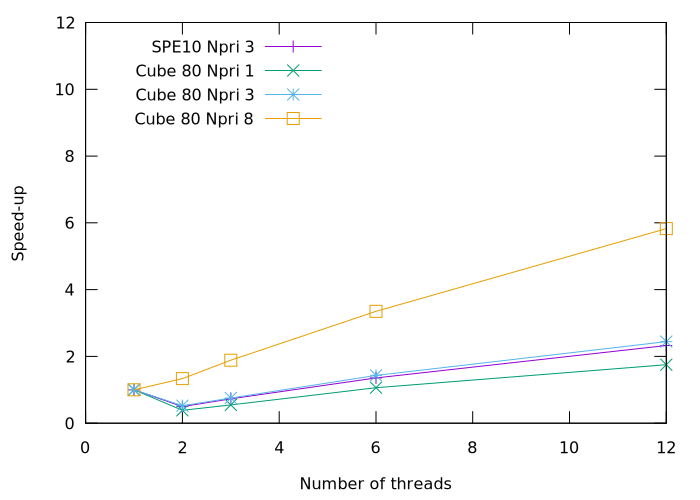
\includegraphics[width=0.6\textwidth]{res_facto_no_agg}
  \caption{}
  \label{fig:res_facto_no_agg}
\end{figure}
